\chapter[Constructing IPFs for Medical Images: A Segmentation Problem]{Constructing IPFs for Medical Images:\\A Segmentation Problem}

%---
\section{Chapter Overview}

In Chapter~\ref{chap:ipfs}, the image partition forest (IPF) data structure was introduced, together with an accompanying set of algorithms. This chapter looks at how IPFs can be constructed from medical image slices (2D) or volumes (3D) by adapting the morphological watershed and waterfall algorithms \cite{beucher94,marcotegui05}. This forms the backdrop for Chapter~\ref{chap:featureid}, which describes IPF algorithms for performing automatic feature identification.

%---
\section{The Watershed Transform}

\subsection{Overview}

\iffalse

The grey-scale watershed transform is an image segmentation algorithm which takes a grey-scale image (whether 2D or 3D) as input and produces a partition of that image into regions, one for each local minimum in the image. For the purposes of IPF construction, it is used to construct the leaf layer of the forest, as will be explained later. The algorithm treats an image as a height map. In 2D, this resembles a landscape, as shown in Figure~\ref{fig:segmentation-watershed-landscapeanalogy}.

\fi

The grey-scale watershed transform is an image segmentation algorithm which takes a grey-scale image (whether 2D or 3D) as input and produces a partition of that image into regions, one for each local minimum in the image. It does this by simulating a process of flooding that starts with a pool of water at each local minimum. As the algorithm proceeds, these pools grow, until some of them are on the point of touching each other. At this point, watersheds (dams) are added to keep the pools apart: in segmentation terms, these will become region boundaries, which in turn will yield a partition of the original image into regions associated with its local minima.

%---
\stufigex{height=5cm}{segmentation-watershed-landscapeanalogy.png}{The landscape analogy: Viewing a 2D image as a 3D terrain}{fig:segmentation-watershed-landscapeanalogy}{t}
%---

The process is most easily visualized in 2D. An image $I$ may be considered as a height map, or landscape, as shown in Figure~\ref{fig:segmentation-watershed-landscapeanalogy}: for every point $(x,y)$ in the domain of the image, there is an associated pixel value $I(x,y)$ which gives the height of the landscape at that point. In the 8-bit image shown, for instance, black pixels in the image correspond to a height of $0$ and white pixels correspond to a height of $255$. The watershed process involves metaphorically taking this surface, poking holes through its local minima and lowering it perpendicularly into a lake. As the water rises, the pools of water, or catchment basins, associated with the local minima grow (see Figure~\ref{fig:segmentation-watershed-construction}(a)). Eventually, these catchment basins will meet (Figure~\ref{fig:segmentation-watershed-construction}(b)) and a watershed will be constructed to keep them apart (Figure~\ref{fig:segmentation-watershed-construction}(c)). This process continues until the water has reached the top of the landscape, at which point the algorithm terminates. The watersheds generated during the process divide the landscape into the valleys associated with its local minima, which is equivalent to dividing the base image into regions.

%---
\begin{figure}[t]
\begin{center}
	\subfigure[Beginning the flooding]{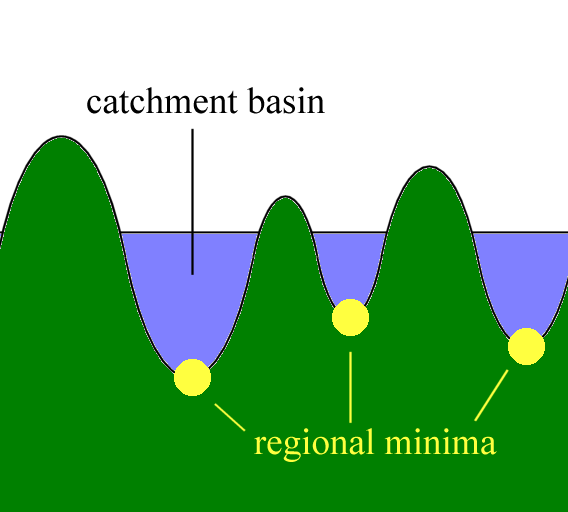
\includegraphics[height=6cm]{segmentation-watershed-construction1.png}}%
	\hspace{4mm}%
	\subfigure[Two catchment basins meet]{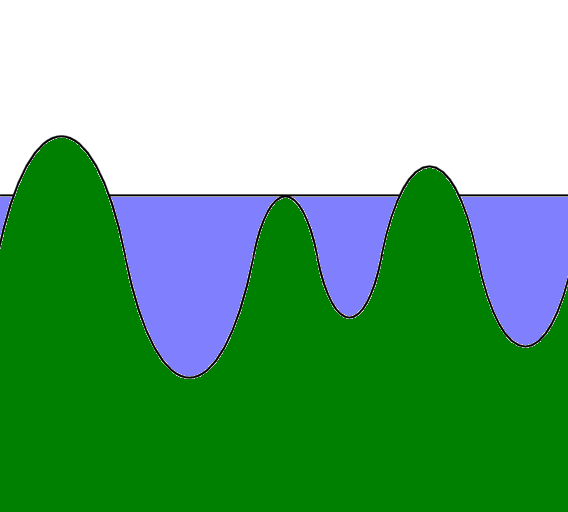
\includegraphics[height=6cm]{segmentation-watershed-construction2.png}}%
	\hspace{4mm}%
	\subfigure[Building a watershed at the join point]{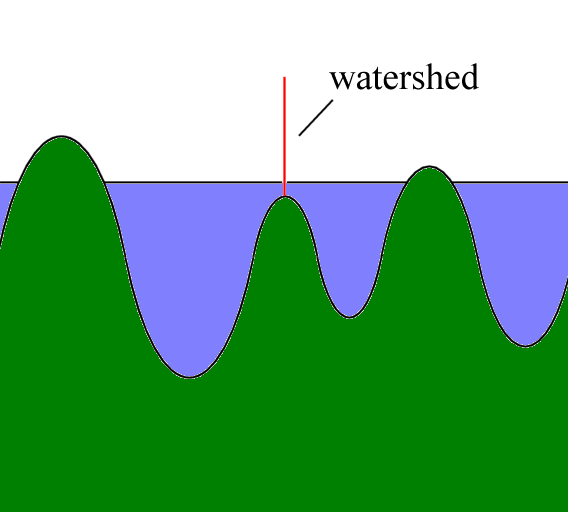
\includegraphics[height=6cm]{segmentation-watershed-construction3.png}}%
	\hspace{4mm}%
	\subfigure[The final division into regions]{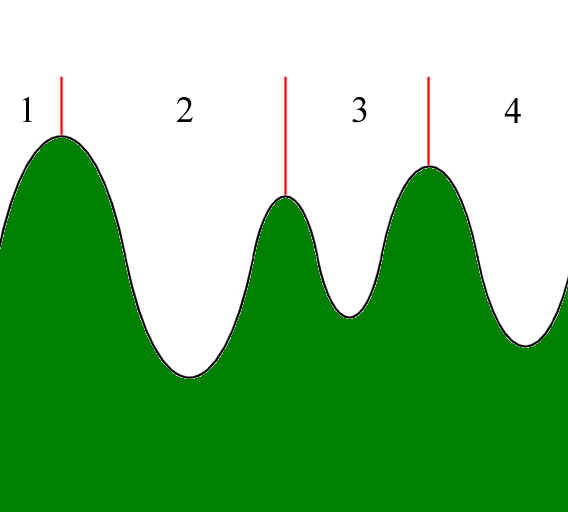
\includegraphics[height=6cm]{segmentation-watershed-construction4.png}}%
\end{center}
\caption{The watershed construction process}
\label{fig:segmentation-watershed-construction}
\end{figure}
%---

\subsection{Definitions}

Formally, an image is considered to be a function $f: \Omega_{\subset \mathbb{Z}^n} \to \mathbb{Z}$ that maps elements of the domain $\Omega$ to integer grey values. (For instance, a $2$-dimensional $512 \times 512$ image could be defined to have domain $\Omega = \{(x,y) : 0 \le x,y < 512\}$.) A pixel $\mathbf{p} \in \Omega$ is defined to have height $f(\mathbf{p})$ and neighbour set $N(\mathbf{p})$, according to some implementation-defined notion of neighbourhood: usually neighbourhood is defined so that pixels are either 4- or 8-connected in 2D, and 6- or 26-connected in 3D (see Figure~\ref{?}).

% TODO: Figure here

A \smgidx[singular minimum]{singular minimum} of an image is a point whose neighbours are all strictly higher than it. Formally, $\mathbf{p}$ is a singular minimum iff $\forall \mathbf{p'} \in N(\mathbf{p}) \cdot f(\mathbf{p'} > f(\mathbf{p})$. A \smgidx[plateau]{plateau} of an image is a maximal set of two or more connected pixels of equal altitude. A \smgidx[plateau!minimal]{minimal plateau} is a plateau from which it is impossible to descend, and a \smgidx[plateau!non-minimal]{non-minimal plateau} is the opposite. Together, the singular minima and minimal plateaux of an image form the \smgidx[local minimum!of image]{local minima} of the image.

TODO

%---
\section{The Waterfall Algorithm}

TODO
